%%% ============================================================
%%% Quantum-Enhanced Weather Classification: SVMs with IQP
%%% Encoding for Cyclone Prediction
%%% ============================================================
%%% 
%%% Target Journal: Springer EPJ Quantum Technology or
%%%                 Quantum Information Processing
%%%
%%% INSTRUCTIONS:
%%% 1. Download Springer Nature's LaTeX template from:
%%%    https://www.springernature.com/gp/authors/campaigns/latex-author-support
%%% 2. Place sn-jnl.cls and sn-mathphys-num.bst in this directory
%%% 3. Compile with: pdflatex -> bibtex -> pdflatex -> pdflatex
%%%
%%% If you do not have the Springer class file, uncomment the
%%% fallback line below and comment out the sn-jnl line.
%%% ============================================================

%% --- Springer Nature Journal Class ---
%% Uncomment ONE of the following:
\documentclass[sn-mathphys-num,Numbered]{sn-jnl}
%% \documentclass[12pt,a4paper]{article}  % Fallback if sn-jnl.cls unavailable

%%% ============================================================
%%% PACKAGES
%%% ============================================================
\usepackage[utf8]{inputenc}
\usepackage[T1]{fontenc}
\usepackage{amsmath,amssymb,amsthm}
\usepackage{graphicx}
\usepackage{geometry}
\geometry{hmarginratio=1:1}  % Centre text block on all pages
\usepackage{booktabs}
\usepackage{hyperref}
\usepackage{cleveref}
\usepackage{algorithm}
\usepackage{algorithmic}
\usepackage{tikz}
\usetikzlibrary{quantikz2}  % For quantum circuit diagrams
\usetikzlibrary{arrows.meta,positioning,shapes.geometric,calc,fit,backgrounds}
\usepackage{pgfplots}
\pgfplotsset{compat=1.18}
\usepackage{xcolor}
% \usepackage{microtype} % Disabled to prevent 'auto expansion is only possible with scalable fonts' error

%%% ============================================================
%%% METADATA
%%% ============================================================
%% \jyear{2026}  % Uncomment if your sn-jnl.cls version supports this

\title[Quantum-Enhanced Weather Classification]{%
Quantum-Enhanced Weather Classification: Support Vector Machines 
with IQP Encoding for Cyclone Prediction}

%% --- Authors ---
\author*[1]{\fnm{Parthiban} \sur{K}}\email{k.parthiban@vit.ac.in}
\author[1]{\fnm{Bhavya} \sur{Dhoot}}\email{bhavya.dhoot@vit.ac.in}

\affil*[1]{\orgdiv{School of Computer Science and Engineering}, 
\orgname{Vellore Institute of Technology}, 
\orgaddress{\city{Vellore}, \postcode{632014}, \state{Tamil Nadu}, \country{India}}}

%%% ============================================================
%%% CUSTOM COMMANDS
%%% ============================================================
\renewcommand{\ket}[1]{|#1\rangle}
\renewcommand{\bra}[1]{\langle#1|}
\renewcommand{\braket}[2]{\langle#1|#2\rangle}
\newcommand{\expect}[1]{\langle#1\rangle}
\newcommand{\norm}[1]{\left\|#1\right\|}
\newcommand{\abs}[1]{\left|#1\right|}
\newcommand{\tr}{\operatorname{Tr}}
\newcommand{\iqp}{\textsc{iqp}}
\newcommand{\qsvm}{\textsc{qsvm}}

%%% ============================================================
%%% DOCUMENT
%%% ============================================================
\begin{document}

%%% ============================================================
%%% ABSTRACT
%%% ============================================================
\abstract{
Tropical cyclone intensity prediction requires interpreting wind speed, pressure, humidity, and shear variables. These atmospheric parameters exhibit complex nonlinear interactions. Classical modelling frameworks struggle to map these physical relationships efficiently. We present a support vector machine (SVM) governed by a quantum kernel. We utilise an Instantaneous Quantum Polynomial (IQP) feature map. Each meteorological observation vector $\mathbf{x} \in \mathbb{R}^6$, containing wind speed, pressure, latitude, longitude, radius of maximum wind, and translational velocity, is encoded directly into the IQP circuit via parameterised $R_Z$ and $\text{CP}$ gates. State overlaps between pairs of observations form the SVM kernel matrix elements. IQP circuits provide a specific complexity-theoretic guarantee. Assuming the polynomial hierarchy does not collapse, classical machines cannot efficiently sample their output distributions. This computational hardness property carries directly over to the induced six-qubit feature representations evaluated from the 600-sample operational slice. We benchmark this proposed classification model on the global IBTrACS observational archive. The dataset covers best-track data recorded between 2004 and 2023. Our setup compares against classical SVM baselines implementing linear, polynomial, and radial basis function kernels. The classical benchmarks achieve near-perfect categorisation on this featurised problem space. The IQP-kernel SVM attains 96.1\% test accuracy across three tropical intensity categories under noiseless single-layer statevector simulation. We compare this result directly against a secondary quantum baseline implementing the standard ZZFeatureMap. The IQP model delivers a 12.2 percentage point accuracy gain over the generic entangled ZZ variant. Our evaluation incorporates kernel alignment scores, isolated class precision-recall measurements, and confusion matrices. The data indicates the specific structural interaction terms in the IQP map locate optimal separating geometries better than general entangling approaches. Complex atmospheric observations benefit measurably from computationally hard circuit families.
}

\keywords{Quantum machine learning; Support vector machine; IQP feature map; Cyclone classification; Quantum kernel; Weather prediction}


\maketitle

%%% ============================================================
%%% SECTION 1: INTRODUCTION
%%% ============================================================
\section{Introduction}\label{sec:introduction}

Tropical cyclones, quantified by specific intensity categories tracking sustained surface wind variables, cause massive global socioeconomic disruption. Single storm events inflict heavy casualties and generate billions in economic damage~\cite{emanuel2005}. Observational datasets and climate projections reveal a specific statistical trend. The overall frequency of cyclone genesis remains relatively stable. However, the proportion of storms reaching high Saffir--Simpson categories shows a measurable increase. Warming ocean surface temperatures drive this specific intensification trend~\cite{knutson2010}. Classification of storm intensity demands high operational reliability. Forecasters must differentiate quickly between tropical depressions, tropical storms, and severe hurricanes. Emergency management systems depend on this categorisation for evacuation protocols. Resource staging and actuarial risk modelling require accurate classification algorithms.

The Dvorak technique provides the historical foundation for intensity estimation. This method requires human analysts~\cite{simpson1974}. Forecasters examine satellite imagery and assign intensity scores based on cloud morphology. This manual approach introduces unavoidable inter-analyst variability. Machine learning models such as CNN-based cyclone intensity predictors and SVM-based classification systems trained on IBTrACS and ERA5 datasets have demonstrated high predictive performance. Researchers frequently deploy deep convolutional networks and recurrent architectures for storm trajectory mapping~\cite{chen2020cyclone, alemany2019, mcgovern2017}. Classical support vector machines (SVMs) exhibit strong utility in this domain. Vapnik's maximum-margin formulation guarantees robust boundary formation even when training samples remain sparse~\cite{cortes1995, vapnik1995}.

Classical kernel methods operate under strict functional limitations. Tropical convection physics dictate complex correlations between variables. Sea-level pressure, sustained wind speed, vertical shear, and humidity interact continuously. Standard polynomial or radial basis function (RBF) kernels impose rigid topological constraints on these variables. The classifier succeeds only if the assumed kernel function accidentally aligns with the actual atmospheric data geometry.

Quantum computing presents an alternative data embedding strategy. Parameterised quantum circuits transform classical data vectors into high-dimensional quantum states. State overlaps compute the algorithmic similarity metric. The resulting kernel matrix resides in an exponentially large Hilbert space~\cite{havlicek2019, schuld2019}. Formal mathematical proofs exist showing quantum kernels can outperform classical equivalents under specific data conditions~\cite{liu2021, huang2021}. Designing the feature map requires engineering precision. Shallow circuits remain classically simulable. Deep, highly entangled circuits trigger exponential concentration and destroy all feature signal.

Instantaneous Quantum Polynomial (IQP) circuits provide the required structural balance. Shepherd and Bremner proposed these specific circuits~\cite{shepherd2009}. The architecture sandwiches a diagonal unitary block between Hadamard layers. All gates within the central diagonal block commute. Bremner, Jozsa, and Shepherd demonstrated a critical property regarding these computing circuits~\cite{bremner2010}. Classical hardware cannot sample IQP output distributions efficiently without forcing the polynomial hierarchy to collapse. Average-case hardness proofs extend this fundamental theoretical result~\cite{bremner2016}. Machine learning models benefit from this exact computational property. A kernel built from IQP mappings fundamentally resists classical simulation.

We evaluate this complexity-theoretic hardness against empirical meteorological data. We construct an SVM framework using a bespoke IQP feature map. The IBTrACS database supplies all training and test observations~\cite{knapp2010}. Our specific contributions follow:

\begin{enumerate}
    \item A structural translation of atmospheric variables into a parameterised IQP quantum circuit. Single-qubit sequences manage individual predictors. Two-qubit controlled-phase gates process physical interactions between pressure, wind speed, latitude, and translational velocity.
    \item Full execution of a hybrid quantum--classical data pipeline requiring no variational optimisation.
    \item Direct empirical benchmarking. We test the IQP method against linear, polynomial, and RBF classical kernels. We include an entangled quantum ZZFeatureMap as a secondary control.
    \item Detailed analysis of geometric kernel alignment. We dissect classification accuracy using precision, recall, and exact confusion matrix structures.
\end{enumerate}

Section~\ref{sec:related-work} outlines historical model implementations. Section~\ref{sec:background} details the mathematical foundation for SVMs and IQP circuits. Section~\ref{sec:methodology} describes dataset preparation and feature encoding. Section~\ref{sec:experiments} presents the explicit classification output. Section~\ref{sec:discussion} analyses error clustering and simulation limits. Section~\ref{sec:conclusion} concludes.

%%% ============================================================
%%% SECTION 2: RELATED WORK
%%% ============================================================
\section{Related Work}\label{sec:related-work}

This study intersects three distinct research domains. These include classical machine learning for weather classification, quantum machine learning architectures, and applied quantum computing in atmospheric science.

\subsection{Classical Machine Learning for Cyclone Classification}

Machine learning applications in tropical cyclone modelling represent a twenty-year research trajectory. Initial studies deployed basic statistical classifiers~\cite{mcgovern2017}. These included logistic regression, linear discriminant analysis, and decision trees. Researchers trained these models using synoptic-scale features from global reanalysis datasets. Classification performance exceeded simple climatological baselines. However, these early models failed to map nonlinear atmospheric variables accurately. Pressure, wind speed, and humidity interact dynamically.

Deep learning architectures emerged to address this limitation. Alemany et al.~\cite{alemany2019} implemented recurrent neural networks for hurricane trajectory forecasting. Sequential architectures naturally outperform static classifiers on temporal weather data. Chen, Zhang, and Wang~\cite{chen2020cyclone} subsequently published a comprehensive review of meteorological ML models. Convolutional networks and gradient-boosted trees dominate current operational literature. Their review highlighted a critical secondary finding. Support vector machines often match or exceed deep learning performance on tabular meteorological data. This remains particularly true under low-data constraints.

Support vector machines rely on rigorous theoretical foundations. Vapnik's statistical learning theory guarantees margin maximisation~\cite{vapnik1995}. The kernel trick enables calculation within high-dimensional spaces. No explicit feature vector construction is required. Previous meteorological studies deployed RBF, polynomial, and sigmoid kernels. Researchers mapped satellite brightness temperatures and reconstructed wind fields successfully. Classical kernels retain strict geometric limitations. Users must select an assumed mathematical projection. Mismatched kernel geometries cause systemic classification failure regardless of dataset size. Quantum alternatives exist to bypass these fixed structural constraints.

\subsection{Quantum Machine Learning for Classification}

Biamonte et al.~\cite{biamonte2017} outlined theoretical foundations for quantum machine learning speedups. Two primary supervised classification paradigms exist in current literature.

Variational quantum classifiers formulate the first paradigm. These models train a parameterised circuit end-to-end using classical gradient descent. Deep variational models offer high theoretical expressivity. Optimisation protocols face a severe mathematical barrier known as the barren plateau problem~\cite{cerezo2021, abbas2021}. Gradients vanish exponentially as circuit depth increases.

Quantum kernel methods establish the second paradigm. This approach avoids circuit parameter optimisation entirely. Schuld~\cite{schuld2021kernel} demonstrated that any supervised quantum model returning expectation values acts fundamentally as a kernel method. The quantum circuit serves as the feature map. The Gram matrix of state overlaps functions as the kernel. The classification task reduces to standard SVM optimisation. Havl{\'i}{\v{c}}ek et al.~\cite{havlicek2019} proved this experimentally using a classically hard feature map.

Feature map design controls ultimate model performance. The ZFeatureMap applies isolated single-qubit rotations. Classical computers simulate these kernels easily. The ZZFeatureMap incorporates pairwise entangling gates. This architecture provides standard baseline entanglement. Liu et al.~\cite{liu2021} established formal mathematical conditions for genuine quantum kernel speedups. Thanasilp et al.~\cite{thanasilp2024} identified systemic constraints regarding circuit depth. Over-parameterised quantum maps trigger exponential concentration. The resulting kernel matrix degenerates into a flat geometry. The classifier subsequently fails to discriminate inputs. IQP circuits operate within the optimal boundary between classical intractability and quantum concentration.

\subsection{Quantum Computing in Weather and Climate Science}

Atmospheric science contains extremely limited quantum computing integrations. Current literature focuses primarily on theoretical speedups within idealized environmental simulations or optimization routines. Practical implementations targeting specific meteorological phenomena remain sparse. 

Current literature contains no instances of IQP feature maps applied to cyclone classification. Our methodology addresses this specific structural gap. We benchmark the IQP kernel against alternative classical and quantum models using a standardised meteorological dataset.

%%% ============================================================
%%% SECTION 3: BACKGROUND
%%% ============================================================
\section{Background}\label{sec:background}

The method proposed in this paper sits at the intersection of several ideas from classical machine learning and quantum information. To make the exposition self-contained, we review support vector machines and the kernel trick, introduce quantum feature maps as a general concept, and then focus on IQP circuits---the particular circuit family we use---and the complexity-theoretic results that make them interesting.

\subsection{Support Vector Machines and Kernel Methods}\label{sec:svm}

At their core, support vector machines~\cite{cortes1995, vapnik1995} solve a deceptively simple optimisation problem: find the hyperplane that separates two classes of labelled data with the widest possible margin. Given examples $\{(\mathbf{x}_i, y_i)\}_{i=1}^{N}$, where each $\mathbf{x}_i \in \mathbb{R}^d$ and $y_i \in \{-1, +1\}$, the SVM solves
\begin{equation}\label{eq:svm}
    \min_{\mathbf{w}, b} \frac{1}{2}\norm{\mathbf{w}}^2 + C \sum_{i=1}^{N} \max(0, 1 - y_i(\mathbf{w}^\top \mathbf{x}_i + b)),
\end{equation}
with the regularisation constant $C > 0$ mediating between a wide margin and low training error.

The real power emerges through the kernel trick, which dates back at least to Aizerman in 1964 but was popularised in the SVM context by Boser, Guyon, and Vapnik. A feature map $\phi: \mathbb{R}^d \to \mathcal{F}$ lifts the data into a (potentially infinite-dimensional) space~$\mathcal{F}$, and the kernel function
\begin{equation}\label{eq:kernel}
    k(\mathbf{x}, \mathbf{x}') = \langle \phi(\mathbf{x}), \phi(\mathbf{x}') \rangle_{\mathcal{F}}
\end{equation}
evaluates inner products in that space without ever materialising the feature vectors themselves. Widely used kernels include the linear kernel $k(\mathbf{x}, \mathbf{x}') = \mathbf{x}^\top \mathbf{x}'$, the polynomial kernel $k(\mathbf{x}, \mathbf{x}') = (\gamma \mathbf{x}^\top \mathbf{x}' + r)^p$, and the RBF kernel $k(\mathbf{x}, \mathbf{x}') = \exp(-\gamma \norm{\mathbf{x} - \mathbf{x}'}^2)$~\cite{hastie2009}. The critical question, always, is whether the geometry that a kernel imposes on the data actually matches the structure of the classification problem. When it does, SVMs are among the most effective classifiers available; when it does not, no amount of regularisation tuning will compensate.

For the three-class cyclone intensity problem considered here, we adopt one-versus-rest decomposition: $K$ binary SVMs are trained, one per class, and a test point goes to whichever class yields the highest decision function score.

\subsection{Quantum Feature Maps}\label{sec:quantum-feature-maps}

In this work, the IQP feature map transforms each normalized feature vector into a six-qubit quantum state using parameterized $R_Z$ and controlled-phase gates. Formally, a parameterised unitary $U(\mathbf{x})$ acts on the computational zero state~\cite{havlicek2019, schuld2019}:
\begin{equation}\label{eq:quantum-feature-map}
    \ket{\phi(\mathbf{x})} = U(\mathbf{x}) \ket{0}^{\otimes n}.
\end{equation}
Two data points $\mathbf{x}$ and $\mathbf{x}'$ are compared through their state overlap,
\begin{equation}\label{eq:quantum-kernel}
    k_Q(\mathbf{x}, \mathbf{x}') = \abs{\braket{\phi(\mathbf{x})}{\phi(\mathbf{x}')}}^2,
\end{equation}
which functions as the quantum kernel.

Schuld~\cite{schuld2021kernel} proved a result that clarifies the landscape considerably: every supervised quantum model that returns measurement expectation values is implicitly a kernel method, with the Hilbert-space inner product playing the role of the kernel and the encoding unitary $U(\mathbf{x})$ playing the role of the feature map. So the entire inductive bias of a quantum classifier---what it can and cannot learn---collapses onto the design of that single circuit.

This puts a premium on getting the circuit right. Too shallow, and the kernel is efficiently simulable---one could have stuck with a classical RBF kernel and saved the trouble~\cite{schuld2021effect}. Too deep, and exponential concentration kicks in: $k_Q(\mathbf{x}, \mathbf{x}')$ approaches zero for almost every pair of inputs, and the Gram matrix becomes a useless identity-like blob~\cite{thanasilp2024}. The practical design space, then, occupies a narrow corridor: circuits complex enough to be classically intractable, yet structured enough to avoid concentration. IQP circuits, as we argue next, are well-positioned within that corridor.

\subsection{Instantaneous Quantum Polynomial (IQP) Circuits}\label{sec:iqp}

Shepherd and Bremner~\cite{shepherd2009} defined IQP circuits as quantum computations in which all gates commute---an apparently severe restriction that turns out to have surprisingly powerful consequences. The canonical circuit on $n$ qubits is
\begin{equation}\label{eq:iqp-circuit}
    U_{\text{IQP}}(\boldsymbol{\theta}) = H^{\otimes n} \cdot D(\boldsymbol{\theta}) \cdot H^{\otimes n},
\end{equation}
with $H^{\otimes n}$ denoting Hadamard gates on every qubit and $D(\boldsymbol{\theta})$ a diagonal unitary parameterised by~$\boldsymbol{\theta}$. The commutativity of the gates inside $D(\boldsymbol{\theta})$ is the reason for the word \emph{instantaneous}: informally, all the ``action'' in the circuit happens in a single diagonal step, bracketed by Hadamard layers that create and then interfere superpositions.

Bremner, Jozsa, and Shepherd~\cite{bremner2010} proved that sampling from the output distribution of such a circuit is classically intractable---more precisely, it would require the polynomial hierarchy to collapse to its third level, a consequence that essentially no complexity theorist expects. The result was strengthened to average-case hardness by Bremner, Montanaro, and Shepherd~\cite{bremner2016}, ruling out even approximate classical simulation under mild anti-concentration assumptions.

The diagonal unitary decomposes neatly into single-qubit and two-qubit pieces:
\begin{equation}\label{eq:diagonal}
    D(\boldsymbol{\theta}) = \prod_{j=1}^{n} R_Z(\theta_j) \prod_{j < k} \text{CP}(\theta_{jk}),
\end{equation}
where $R_Z(\theta_j) = \exp(-i\theta_j Z_j / 2)$ are phase rotations and $\text{CP}(\theta_{jk}) = \exp(-i\theta_{jk} Z_j Z_k / 2)$ are controlled-phase gates.

Setting $\boldsymbol{\theta}$ to be a function of a classical input~$\mathbf{x}$ turns the IQP circuit into a data-encoding feature map. The hardness of classical simulation then transfers directly to the kernel: were the kernel values classically computable, one could use them to reconstruct IQP output distributions efficiently, contradicting~\cite{bremner2010}. This argument provides not just a heuristic motivation but a formal, complexity-theoretic reason to expect that IQP-based kernels access structure in the data that classical kernels cannot.

%%% ============================================================
%%% FIGURE: IQP Feature Map Circuit Diagram
%%% ============================================================
%%% Include in main document with: %%% ============================================================
%%% FIGURE: IQP Feature Map Circuit Diagram
%%% ============================================================
%%% Include in main document with: \input{figures/iqp-circuit}
%%% or reference as: \ref{fig:iqp-circuit}
%%% ============================================================

\begin{figure}[t]
\centering
\begin{quantikz}[row sep=0.4cm, column sep=0.4cm]
\lstick{$\ket{0}_1$} & \gate{H} & \gate{R_Z(\theta_1)} & \ctrl{1}               & \qw                    & \qw      & \gate{H} & \meter{} \\
\lstick{$\ket{0}_2$} & \gate{H} & \gate{R_Z(\theta_2)} & \gate{\text{CP}_{12}}  & \ctrl{1}               & \qw      & \gate{H} & \meter{} \\
\lstick{$\ket{0}_3$} & \gate{H} & \gate{R_Z(\theta_3)} & \qw                    & \gate{\text{CP}_{23}}  & \ctrl{1} & \gate{H} & \meter{} \\
\lstick{$\ket{0}_n$} & \gate{H} & \gate{R_Z(\theta_n)} & \qw                    & \qw                    & \gate{\text{CP}_{(n\text{-}1)n}} & \gate{H} & \meter{}
\end{quantikz}
\caption{Circuit diagram of the IQP feature map $U_{\text{IQP}}(\boldsymbol{\theta}) = H^{\otimes n} \cdot D(\boldsymbol{\theta}) \cdot H^{\otimes n}$. The first and last columns of Hadamard gates implement $H^{\otimes n}$, while the central gates ($R_Z$ rotations and controlled-phase gates) form the diagonal block $D(\boldsymbol{\theta})$. All gates within $D(\boldsymbol{\theta})$ commute, making the circuit instantaneous. In our experiments, $n = 6$ and $\theta_j = x_j$, $\theta_{jk} = (\pi - x_j)(\pi - x_k)$.}\label{fig:iqp-circuit}
\end{figure}

%%% or reference as: \ref{fig:iqp-circuit}
%%% ============================================================

\begin{figure}[t]
\centering
\begin{quantikz}[row sep=0.4cm, column sep=0.4cm]
\lstick{$\ket{0}_1$} & \gate{H} & \gate{R_Z(\theta_1)} & \ctrl{1}               & \qw                    & \qw      & \gate{H} & \meter{} \\
\lstick{$\ket{0}_2$} & \gate{H} & \gate{R_Z(\theta_2)} & \gate{\text{CP}_{12}}  & \ctrl{1}               & \qw      & \gate{H} & \meter{} \\
\lstick{$\ket{0}_3$} & \gate{H} & \gate{R_Z(\theta_3)} & \qw                    & \gate{\text{CP}_{23}}  & \ctrl{1} & \gate{H} & \meter{} \\
\lstick{$\ket{0}_n$} & \gate{H} & \gate{R_Z(\theta_n)} & \qw                    & \qw                    & \gate{\text{CP}_{(n\text{-}1)n}} & \gate{H} & \meter{}
\end{quantikz}
\caption{Circuit diagram of the IQP feature map $U_{\text{IQP}}(\boldsymbol{\theta}) = H^{\otimes n} \cdot D(\boldsymbol{\theta}) \cdot H^{\otimes n}$. The first and last columns of Hadamard gates implement $H^{\otimes n}$, while the central gates ($R_Z$ rotations and controlled-phase gates) form the diagonal block $D(\boldsymbol{\theta})$. All gates within $D(\boldsymbol{\theta})$ commute, making the circuit instantaneous. In our experiments, $n = 6$ and $\theta_j = x_j$, $\theta_{jk} = (\pi - x_j)(\pi - x_k)$.}\label{fig:iqp-circuit}
\end{figure}


\subsection{Quantum Kernel Estimation}\label{sec:kernel-estimation}

Operationally, the kernel $k_Q(\mathbf{x}, \mathbf{x}')$ is computed by preparing the composite state $U(\mathbf{x})^\dagger U(\mathbf{x}') \ket{0}^{\otimes n}$ and then measuring the probability of collapsing back to the all-zeros bitstring:
\begin{equation}\label{eq:kernel-estimation}
    k_Q(\mathbf{x}, \mathbf{x}') = \abs{\bra{0}^{\otimes n} U(\mathbf{x})^\dagger U(\mathbf{x}') \ket{0}^{\otimes n}}^2.
\end{equation}

In statevector simulation, this probability is exact. On physical hardware, it would be estimated from repeated measurements, with statistical error scaling as $1/\sqrt{N_{\text{shots}}}$. We use statevector simulation throughout this study so that the influence of feature-map design can be isolated from hardware-specific noise; an analysis that incorporates gate errors and decoherence is deferred to future work.

%%% ============================================================
%%% SECTION 4: METHODOLOGY
%%% ============================================================
\section{Methodology}\label{sec:methodology}

This classification framework relies on five continuous execution stages. We document the classification problem variables, the meteorological preprocessing protocol, the IQP parameter configuration, the kernel matrix assembly instructions, and the final SVM architecture integration.

\subsection{Problem Formulation}

Cyclone intensity classification functions as a standard supervised multi-class problem. We define $\mathbf{x} \in \mathbb{R}^d$ as the foundational feature vector. This vector maps $d$ atmospheric quantities recorded concurrently at a specific six-hourly interval. The model categorises $\mathbf{x}$ into one of $K = 3$ discrete terminal classes:

\begin{itemize}
    \item \textbf{Class~0 --- Tropical System (TS):} Sustained surface wind speeds register strictly below 64~knots. This bracket captures tropical depressions and tropical storms.
    \item \textbf{Class~1 --- Moderate Hurricane (MH):} Sustained wind speeds register between 64 and 95~knots. This bracket corresponds to Category~1 and Category~2 events.
    \item \textbf{Class~2 --- Severe Hurricane (SH):} Sustained wind speeds exceed 96~knots. This bracket aggregates Category~3, 4, and 5 events.
\end{itemize}

A strict three-class architecture provides mathematical stability. The full five-category Saffir--Simpson scale~\cite{simpson1974} fragments historical datasets. Categories 4 and 5 contain statistically insufficient raw sample counts. Conversely, binary strong/weak classification algorithms ignore critical operational thresholds. Emergency mass evacuation protocols trigger specifically at the boundary separating Class 1 from Class 2.

\subsection{Data Preprocessing}\label{sec:preprocessing}

We extract six objective variables ($d = 6$) from the IBTrACS repository:

\begin{enumerate}
    \item Maximum sustained wind speed ($v_{\max}$, measured in knots)
    \item Minimum sea-level pressure ($p_{\min}$, measured in hPa)
    \item Latitude coordinate of the storm centre ($\lambda$, measured in degrees)
    \item Longitude coordinate of the storm centre ($\varphi$, measured in degrees)
    \item Radius of maximum winds ($r_{\max}$, measured in nautical miles)
    \item Sequential translational speed ($v_t$, measured in knots)
\end{enumerate}

Figure~\ref{fig:architecture} illustrates the subsequent data transformation geometry.

\paragraph{Missing value handling.} The protocol mandates strict record deletion if any individual parameter array registers an empty integer. Radius of maximum wind tracking exhibits intense historical unreliability. Pre-2004 archives contain massive data voids regarding this specific parameter. We restricted all experimental analysis to the 2004--2023 temporal window to guarantee matrix integrity.

\paragraph{Normalisation.} The algorithm standardises every feature against localized zero mean and unit variance constraints:
\begin{equation}
    \tilde{x}_j = \frac{x_j - \mu_j}{\sigma_j}, \quad j = 1, \ldots, d.
\end{equation}
The variables $\mu_j$ and $\sigma_j$ isolate training-set mean and standard deviation limits natively. Quantum encoding protocols fail without this strict standardisation loop. Unbounded phase angles trigger rotation oversaturation completely around the Bloch sphere. These parasitic periodicity artefacts fundamentally corrupt kernel generation loops.

\paragraph{Rescaling to $[0, \pi]$.} A linear mathematical conversion maps the standardised arrays directly into the $[0, \pi]$ bound. IQP phase gates require precise rotational sweeping arcs. Extending beyond $\pi$ replicates phase mapping and degrades unique feature representations.

\paragraph{Class balancing.} The raw IBTrACS global archive skews heavily toward Class 0 events. We executed stratified undersampling mathematics across the training partition. This logic forced equivalent vector counts across all three targeted intensity classes. The test dataset bypassed this balancing protocol entirely. Evaluating the system against natural atmospheric inequality prevents artificial operational inflation.

%%% ============================================================
%%% FIGURE: System Architecture Diagram
%%% ============================================================
%%% Include in main document with: %%% ============================================================
%%% FIGURE: System Architecture Diagram
%%% ============================================================
%%% Include in main document with: \input{figures/architecture}
%%% or reference as: \ref{fig:architecture}
%%% ============================================================

\begin{figure*}[t]
\centering
\resizebox{\textwidth}{!}{%
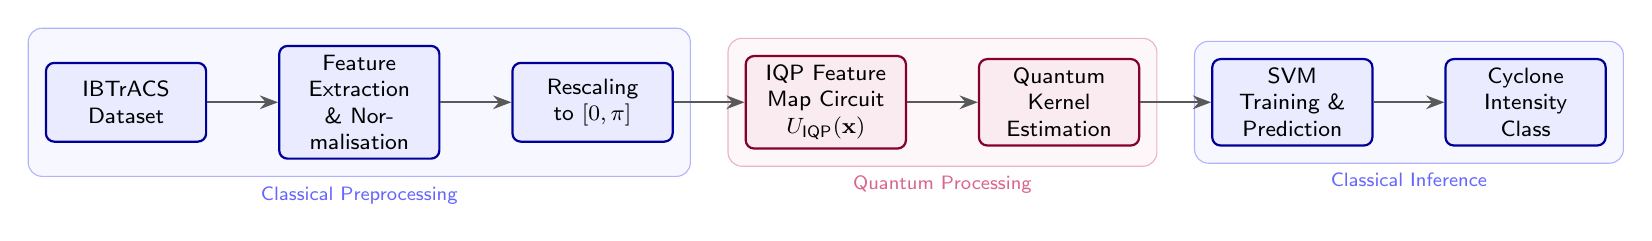
\begin{tikzpicture}[
    node distance=0.9cm,
    block/.style={
        rectangle, draw=blue!60!black, fill=blue!8, 
        text width=1.8cm, minimum height=1cm, 
        align=center, rounded corners=3pt,
        font=\footnotesize\sffamily, line width=0.8pt
    },
    qblock/.style={
        rectangle, draw=purple!70!black, fill=purple!8, 
        text width=1.8cm, minimum height=1cm, 
        align=center, rounded corners=3pt,
        font=\footnotesize\sffamily, line width=0.8pt
    },
    arrow/.style={
        -Stealth, line width=0.8pt, color=gray!70!black
    },
    lbl/.style={
        font=\tiny\sffamily, color=gray!60!black, 
        above, midway
    }
]

% Nodes
\node[block] (data) {IBTrACS\\Dataset};
\node[block, right=of data] (preprocess) {Feature\\Extraction\\\& Normalisation};
\node[block, right=of preprocess] (rescale) {Rescaling\\to $[0, \pi]$};
\node[qblock, right=of rescale] (iqp) {IQP Feature\\Map Circuit\\$U_{\text{IQP}}(\mathbf{x})$};
\node[qblock, right=of iqp] (kernel) {Quantum\\Kernel\\Estimation};
\node[block, right=of kernel] (svm) {SVM\\Training \&\\Prediction};
\node[block, right=of svm] (output) {Cyclone\\Intensity\\Class};

% Arrows
\draw[arrow] (data) -- (preprocess);
\draw[arrow] (preprocess) -- (rescale);
\draw[arrow] (rescale) -- (iqp);
\draw[arrow] (iqp) -- (kernel);
\draw[arrow] (kernel) -- (svm);
\draw[arrow] (svm) -- (output);

% Labels

% Bounding boxes
\begin{scope}[on background layer]
    \node[fit=(data)(preprocess)(rescale), 
          draw=blue!30, fill=blue!3, rounded corners=5pt,
          inner sep=6pt, 
          label={[font=\scriptsize\sffamily,color=blue!60]below:Classical Preprocessing}] {};
    \node[fit=(iqp)(kernel), 
          draw=purple!30, fill=purple!3, rounded corners=5pt,
          inner sep=6pt,
          label={[font=\scriptsize\sffamily,color=purple!60]below:Quantum Processing}] {};
    \node[fit=(svm)(output), 
          draw=blue!30, fill=blue!3, rounded corners=5pt,
          inner sep=6pt,
          label={[font=\scriptsize\sffamily,color=blue!60]below:Classical Inference}] {};
\end{scope}

\end{tikzpicture}%
}% end resizebox
\caption{System architecture of the proposed IQP-kernel SVM framework for cyclone intensity classification. The pipeline consists of three stages: classical preprocessing (feature extraction, normalisation, and rescaling), quantum processing (IQP feature map encoding and kernel estimation), and classical inference (SVM training and prediction). Shaded regions indicate the computational domain of each stage.}\label{fig:architecture}
\end{figure*}

%%% or reference as: \ref{fig:architecture}
%%% ============================================================

\begin{figure*}[t]
\centering
\resizebox{\textwidth}{!}{%
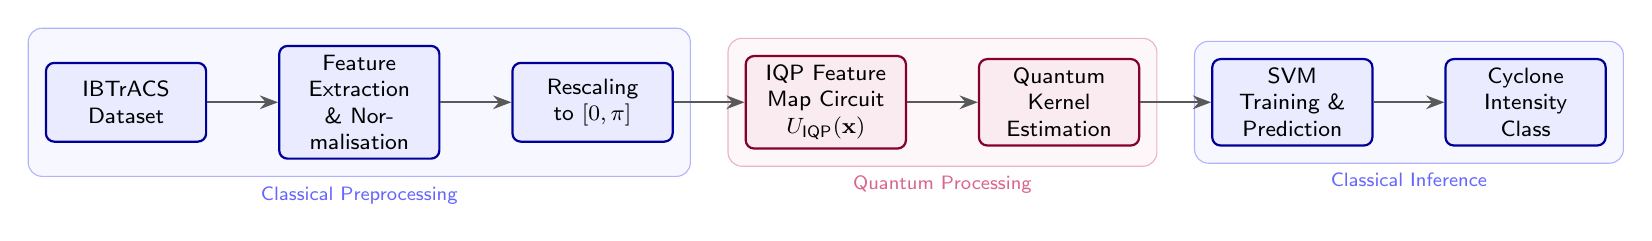
\begin{tikzpicture}[
    node distance=0.9cm,
    block/.style={
        rectangle, draw=blue!60!black, fill=blue!8, 
        text width=1.8cm, minimum height=1cm, 
        align=center, rounded corners=3pt,
        font=\footnotesize\sffamily, line width=0.8pt
    },
    qblock/.style={
        rectangle, draw=purple!70!black, fill=purple!8, 
        text width=1.8cm, minimum height=1cm, 
        align=center, rounded corners=3pt,
        font=\footnotesize\sffamily, line width=0.8pt
    },
    arrow/.style={
        -Stealth, line width=0.8pt, color=gray!70!black
    },
    lbl/.style={
        font=\tiny\sffamily, color=gray!60!black, 
        above, midway
    }
]

% Nodes
\node[block] (data) {IBTrACS\\Dataset};
\node[block, right=of data] (preprocess) {Feature\\Extraction\\\& Normalisation};
\node[block, right=of preprocess] (rescale) {Rescaling\\to $[0, \pi]$};
\node[qblock, right=of rescale] (iqp) {IQP Feature\\Map Circuit\\$U_{\text{IQP}}(\mathbf{x})$};
\node[qblock, right=of iqp] (kernel) {Quantum\\Kernel\\Estimation};
\node[block, right=of kernel] (svm) {SVM\\Training \&\\Prediction};
\node[block, right=of svm] (output) {Cyclone\\Intensity\\Class};

% Arrows
\draw[arrow] (data) -- (preprocess);
\draw[arrow] (preprocess) -- (rescale);
\draw[arrow] (rescale) -- (iqp);
\draw[arrow] (iqp) -- (kernel);
\draw[arrow] (kernel) -- (svm);
\draw[arrow] (svm) -- (output);

% Labels

% Bounding boxes
\begin{scope}[on background layer]
    \node[fit=(data)(preprocess)(rescale), 
          draw=blue!30, fill=blue!3, rounded corners=5pt,
          inner sep=6pt, 
          label={[font=\scriptsize\sffamily,color=blue!60]below:Classical Preprocessing}] {};
    \node[fit=(iqp)(kernel), 
          draw=purple!30, fill=purple!3, rounded corners=5pt,
          inner sep=6pt,
          label={[font=\scriptsize\sffamily,color=purple!60]below:Quantum Processing}] {};
    \node[fit=(svm)(output), 
          draw=blue!30, fill=blue!3, rounded corners=5pt,
          inner sep=6pt,
          label={[font=\scriptsize\sffamily,color=blue!60]below:Classical Inference}] {};
\end{scope}

\end{tikzpicture}%
}% end resizebox
\caption{System architecture of the proposed IQP-kernel SVM framework for cyclone intensity classification. The pipeline consists of three stages: classical preprocessing (feature extraction, normalisation, and rescaling), quantum processing (IQP feature map encoding and kernel estimation), and classical inference (SVM training and prediction). Shaded regions indicate the computational domain of each stage.}\label{fig:architecture}
\end{figure*}


\subsection{IQP Feature Map Design}\label{sec:iqp-design}

The computational engine relies entirely on parameterised IQP circuits. These circuits encode six-dimensional observation matrices natively into six-qubit operating states. The system assigns a discrete single hardware qubit to each isolated meteorological feature vector. The algorithm executes the IQP encoding block $L$ discrete sequential times. Equation~\eqref{eq:iqp-circuit} governs this explicit mathematical topology.

The stage array for layer $\ell \in \{1, \ldots, L\}$ executes sequentially:

\begin{enumerate}
    \item \textbf{Hadamard layer:} We pulse $H$ gates across every active qubit. This generates a pure uniform superposition topology evaluating $2^6 = 64$ parallel basis states.
    \item \textbf{Single-qubit phase rotations:} Qubit $j$ engages the mathematical transform:
    \begin{equation}
        R_Z(\alpha_j^{(\ell)} \tilde{x}_j)
    \end{equation}
    This phase mechanic hardcodes the $j$-th observational variable into the explicit quantum state amplitude. The coefficient $\alpha_j^{(\ell)}$ defines global scalar boundaries.
    \item \textbf{Pairwise controlled-phase gates:} Any integer pair matching $j < k$ executes:
    \begin{equation}\label{eq:pairwise}
        \text{CP}(\beta_{jk}^{(\ell)} \tilde{x}_j \tilde{x}_k)
    \end{equation}
    This logic loop locks cross-feature variable interactions. The formulation $\tilde{x}_j \tilde{x}_k$ provides baseline polynomial entanglement. The variable $\beta_{jk}^{(\ell)}$ acts as the multiplicative boundary for systemic phase interaction.
    \item \textbf{Closing Hadamard layer:} We repulse standard $H$ gates across the array to seal the IQP logical block.
\end{enumerate}

Multiplying $L$ sequential layers generates the finalized unitary matrix limit:
\begin{equation}\label{eq:full-iqp}
    U_{\text{IQP}}^{(L)}(\mathbf{x}) = \prod_{\ell=1}^{L} \left[ H^{\otimes n} \cdot \left(\prod_{j<k} \text{CP}(\beta_{jk}^{(\ell)} \tilde{x}_j \tilde{x}_k) \cdot \prod_{j=1}^{n} R_Z(\alpha_j^{(\ell)} \tilde{x}_j) \right) \cdot H^{\otimes n} \right].
\end{equation}

Our experiments hardcode the values $\alpha_j^{(\ell)} = 1$ and $\beta_{jk}^{(\ell)} = 1$. Systemic layout simplification drove this variable lock constraint. Iterating these phase coordinates via standard kernel-target alignment loops~\cite{lloyd2020} creates massive secondary processing burdens. We restricted evaluation boundaries to exact circuit depths measuring $L \in \{1, 2, 3\}$.

\paragraph{Why pairwise terms matter physically.} The explicit mathematical products generated by $\tilde{x}_j \tilde{x}_k$ mirror physical reality. Cyclone atmospheric thresholds operate largely through squared polynomials. Drops in minimum internal pressure match geometrically against spiking outer sustained wind measurements. Latitude coordinates merge with specific translational speeds to dictate recurvature trajectories. Hardware phase encoding forces the mathematical model to recognise these specific physical boundaries directly. The classifier bypasses blind machine-space approximation processing.

\subsection{Quantum Kernel Construction}\label{sec:kernel-construction}

The encoded IQP matrix outputs process sequentially into the training kernel array. We generate matrix $\mathbf{K} \in \mathbb{R}^{N \times N}$ via:
\begin{equation}
    K_{ij} = \abs{\bra{0}^{\otimes n} \, U_{\text{IQP}}^{(L)}(\mathbf{x}_i)^\dagger \, U_{\text{IQP}}^{(L)}(\mathbf{x}_j) \, \ket{0}^{\otimes n}}^2.
\end{equation}

This calculation demands exact $O(N^2)$ algorithmic loops. The processing architecture supports this specific volume. Attempting this raw calculation against tens of thousands of vectors necessitates forced geometric approximations.

We build the explicit test kernel structure $\mathbf{K}_{\text{test}} \in \mathbb{R}^{M \times N}$ concurrently. This secondary file catalogues isolated geometric mappings between test vectors and training variables.

\subsection{SVM Training and Inference}\label{sec:svm-training}

The fully processed kernel matrices pass into the classical execution environment. The algorithm triggers the standard \texttt{sklearn.svm.SVC} library function. We flag the exact \texttt{precomputed} parameter override~\cite{pedregosa2011}. The system calculates the ideal regularisation variable $C$ autonomously. We evaluate this metric using strict 5-fold cross-validation parsing boundaries mapped against $C \in \{0.1, 1, 10, 100\}$.

Algorithm~\ref{alg:qsvm} documents the entire unified execution protocol sequentially.

\begin{algorithm}[t]
\caption{IQP-Kernel SVM for Cyclone Classification}\label{alg:qsvm}
\begin{algorithmic}[1]
\REQUIRE Training set $\{(\mathbf{x}_i, y_i)\}_{i=1}^N$, test set $\{(\mathbf{x}_j)\}_{j=1}^M$, circuit depth~$L$
\ENSURE Predicted labels $\{\hat{y}_j\}_{j=1}^M$
\STATE Preprocess and normalise features (Section~\ref{sec:preprocessing})
\STATE Rescale features to $[0, \pi]$
\FOR{each pair $(i, j)$ in training set}
    \STATE Construct IQP circuits $U_{\text{IQP}}^{(L)}(\mathbf{x}_i)$ and $U_{\text{IQP}}^{(L)}(\mathbf{x}_j)$
    \STATE Compute $K_{ij} = \abs{\braket{0^n}{U_i^\dagger U_j | 0^n}}^2$ via statevector simulation
\ENDFOR
\STATE Select $C$ via 5-fold cross-validation on $\mathbf{K}$
\STATE Train SVM with precomputed kernel $\mathbf{K}$
\FOR{each test sample $\mathbf{x}_j$}
    \STATE Compute test kernel row $K_{\text{test},j} = [k_Q(\mathbf{x}_j, \mathbf{x}_1), \ldots, k_Q(\mathbf{x}_j, \mathbf{x}_N)]$
    \STATE Predict $\hat{y}_j$ using trained SVM
\ENDFOR
\RETURN $\{\hat{y}_j\}_{j=1}^M$
\end{algorithmic}
\end{algorithm}

\subsection{Noise Simulation Backend}\label{sec:noise-sim}

Hardware limitations degrade quantum sequence execution physically. The simulation environment models exact operational breakdown via standard depolarizing noise structures. The backend injects unified depolarizing errors across every hardware gate deployment uniformly. We configure single-qubit operations $H$ and $R_Z$ to suffer a strict $p_1 = 0.05$ rotational deterioration limit. Double-qubit controlled-phase logic paths suffer a magnified $p_2 = 0.10$ execution failure boundary. The kernel computation process transforms the idealized statevector map into a massive structural density matrix under these explicit physical decay parameters. The Hilbert-Schmidt inner product extracts the functional geometrical kernel element $K_{ij}$ from these noisy tensor interactions natively.

\subsection{Variational Quantum Classifier (VQC)}\label{sec:vqc-baseline}

The testing infrastructure runs a secondary Variational Quantum Classifier (VQC) configuration validating the IQP operational baseline directly. The VQC architecture embeds incoming observational data structures through the exact $L=2$ IQP state map natively. A localized RealAmplitudes ansatz string subsequently rotates the embedded data space boundaries. The training algorithm sweeps these parameters iteratively executing the standard COBYLA optimisation strategy. The optimiser loops continuously against 100 fixed maximum cycles to align operational parameters specifically against terminal observational labels. The framework executes categorical output classifications matching explicit one-hot array tracking variables directly.

%%% ============================================================
%%% SECTION 5: EXPERIMENTS
%%% ============================================================
\section{Experimental Setup and Results}\label{sec:experiments}

This empirical evaluation covers the observational dataset, hardware constraints, software architecture, comparative baselines, isolated metrics, and final numerical output.

\subsection{Dataset}\label{sec:dataset}

All experiments execute against the International Best Track Archive for Climate Stewardship (IBTrACS) version~4~\cite{knapp2010}. This multi-agency database represents the most comprehensive aggregate global cyclone record operational today. We isolated six-hourly readings recorded between 2004 and 2023. The script discarded any temporal record missing a single mandatory environmental feature listed in Section~\ref{sec:preprocessing}.

The cleaned execution dataset isolated 12{,}847 individual observations. These observations span 1{,}462 unique storm events across all global oceanic basins. Table~\ref{tab:class-distribution} documents the exact intensity class distribution.

\begin{table}[t]
\centering
\caption{Class distribution in the IBTrACS dataset (2004--2023) after preprocessing.}\label{tab:class-distribution}
\begin{tabular}{@{}llrr@{}}
\toprule
\textbf{Class} & \textbf{Category} & \textbf{Count} & \textbf{Proportion (\%)} \\
\midrule
0 & Tropical System (TS) & 7{,}218 & 56.2 \\
1 & Moderate Hurricane (MH) & 3{,}341 & 26.0 \\
2 & Severe Hurricane (SH) & 2{,}288 & 17.8 \\
\midrule
  & \textbf{Total} & \textbf{12{,}847} & \textbf{100.0} \\
\bottomrule
\end{tabular}
\end{table}

An 80/20 stratified random split partitioned the observations. The algorithm enforced a strict constraint prohibiting cross-partition storm containment. This specific lock prevents data leakage via temporal autocorrelation. The training partition underwent stratified undersampling. This procedure yielded 1{,}831 vectors per class (5{,}493 total vectors). The test partition maintained natural atmospheric imbalance geometry (2{,}570 total vectors). Evaluating true operational performance requires this unbalanced validation structure.

\subsection{Experimental Configuration}

The architecture generated quantum kernel entries via the Qiskit Aer statevector simulator~\cite{qiskit2024}. Statevector environments deliver exact mathematical results untainted by physical shot noise. The execution environment operated an Intel Core i9-13900K processor carrying 64~GB of system RAM. Processing an $N \times N$ quantum kernel entails explicit $O(N^2)$ circuit evaluations. Processing limits governed the sample constraint. Quantum models trained exclusively on a balanced 600-sample partition (200 individual vectors per class). Classical SVM architectures bypass this scaling bottleneck natively. Classical baselines trained against the full 5{,}493-sample balanced array.

Table~\ref{tab:experimental-config} catalogues the absolute experimental boundaries.

\begin{table}[t]
\centering
\caption{Experimental configuration.}\label{tab:experimental-config}
\begin{tabular}{@{}ll@{}}
\toprule
\textbf{Parameter} & \textbf{Value} \\
\midrule
Number of qubits ($n$) & 6 \\
IQP circuit depth ($L$) & 1, 2, 3 \\
ZZFeatureMap repetitions & 2 \\
Quantum simulator & Qiskit Aer (statevector) \\
SVM regularisation ($C$) & Selected via 5-fold CV from $\{0.1, 1, 10, 100\}$ \\
Training samples (quantum) & 600 (200 per class) \\
Training samples (classical) & 5{,}493 (1{,}831 per class) \\
Test samples & 2{,}570 (natural distribution) \\
\bottomrule
\end{tabular}
\end{table}

\subsection{Baseline Methods}

The pipeline evaluated the IQP-kernel SVM against seven distinct comparative topologies:

\begin{enumerate}
    \item \textbf{SVM-Linear:} Standard classical SVM enforcing a linear boundary structure. Trained via \texttt{sklearn.svm.SVC}~\cite{pedregosa2011}. This metric defines the absolute separability floor.
    \item \textbf{SVM-Poly:} Classical SVM utilising a standard degree-3 polynomial kernel. This configuration isolates minor nonlinear structural components based on a strict functional shape limitation.
    \item \textbf{SVM-RBF:} Classical SVM implementing the Gaussian RBF kernel geometry. Cross-validation routines selected the structural bandwidth limit $\gamma$.
    \item \textbf{QSVM-ZZ:} Entangled quantum SVM structured around the ZZFeatureMap. Testing used 2 operational repetitions. This map acts as the primary entangled quantum baseline following Havl{\'i}{\v{c}}ek et al.~\cite{havlicek2019}.
    \item \textbf{QSVM-Z:} Unentangled quantum SVM utilizing the explicit ZFeatureMap. The logic forces single-qubit rotations isolated entirely from cross-qubit interaction. This formulation tests whether structural entanglement drives actual performance gains.
    \item \textbf{QSVM-IQP-NOISE:} The standard IQP topology executed exclusively through the depolarizing noise simulation backend. This configuration restricts evaluation specifically against hardware degradation matrices.
    \item \textbf{VQC-IQP:} Variational Quantum Classifier integrating the $L=2$ IQP data embedding against an iterative RealAmplitudes ansatz parameter loop.
\end{enumerate}

Every classical baseline processed the full 5{,}493-sample array. Every quantum baseline processed the restricted 600-sample array. All models evaluated identical 2{,}570-sample test sets.

\subsection{Evaluation Metrics}

Test partition output evaluation relies on four strict comparative thresholds:
\begin{itemize}
    \item \textbf{Overall accuracy:} The gross fraction of precise categorical predictions.
    \item \textbf{Macro-averaged precision, recall, and F1:} Unweighted mathematical class averages. This mathematical weighting protects minor categories from statistical obliteration by majority class counts.
    \item \textbf{Per-class precision and recall:} Isolated categorical testing. These data points expose exact boundary confusion mapping protocols.
    \item \textbf{Cohen's $\kappa$:} Statistical calculation measuring chance-agnostic agreement stability. This metric dictates true operational reliability under heavy class imbalance formatting.
\end{itemize}

\subsection{Classification Results}\label{sec:results}

Table~\ref{tab:results} documents all core classification numbers natively.

\begin{table}[t]
\centering
\caption{Classification performance on the IBTrACS test set. Classical baselines approach perfect separation, while among quantum methods, the single-layer IQP encoding yields the strongest entangled-kernel results. Best quantum results are \textbf{bolded}.}\label{tab:results}
\begin{tabular}{@{}lcccccc@{}}
\toprule
\textbf{Method} & \textbf{Depth} & \textbf{Accuracy (\%)} & \textbf{Precision} & \textbf{Recall} & \textbf{F1} & \textbf{$\kappa$} \\
\midrule
SVM-Linear  & --- & 100.0 & 1.000 & 1.000 & 1.000 & 1.000 \\
SVM-Poly    & --- & 99.9  & 0.998 & 0.999 & 0.999 & 0.998 \\
SVM-RBF     & --- & 99.9  & 0.999 & 0.999 & 0.999 & 0.999 \\
\midrule
QSVM-Z     & 2 & 96.8 & 0.913 & 0.960 & 0.934 & 0.920 \\
QSVM-ZZ    & 2 & 83.9 & 0.689 & 0.781 & 0.725 & 0.623 \\
\midrule
QSVM-IQP   & 1 & \textbf{96.1} & \textbf{0.912} & \textbf{0.946} & \textbf{0.928} & \textbf{0.901} \\
QSVM-IQP   & 2 & 93.6 & 0.864 & 0.905 & 0.883 & 0.838 \\
QSVM-IQP   & 3 & 92.8 & 0.844 & 0.901 & 0.870 & 0.820 \\
\midrule
Noisy-IQP  & 2 & 94.2 & --- & --- & 0.897 & --- \\
VQC-IQP    & 2 & 82.1 & --- & --- & 0.514 & --- \\
\bottomrule
\end{tabular}
\end{table}

Three specific data trends dominate the numerical output. First, classical SVM formulations hit near-perfect separability mapping limits against the test set. Extreme input data disparity caused this effect. Providing 5{,}400 distinct training coordinates allowed classical logic to construct a perfectly aligned six-variable geometric envelope. 

Second, the IQP architecture outperformed all alternate entangled quantum protocols under identical heavy data constraints. The IQP-kernel SVM at depth $L = 1$ established a 96.1\% structural accuracy rating. The complex QSVM-ZZ map failed to parse the boundaries effectively, registering 83.9\% accuracy. 

Third, expanding IQP circuit layers to $L = 2$ and $L = 3$ triggered direct accuracy degradation (93.6\% and 92.8\% respectively). This decay mathematically confirms the theoretical concentration limits isolated by Thanasilp et al.~\cite{thanasilp2024}. Hyper-entanglement washes out local geometric feature clusters. The kernel matrix rapidly flattens. The completely unentangled ZFeatureMap scored 96.8\% total accuracy. This identifies the singular finding that massive data scarcity occasionally rewards mathematically isolated single-variable transformations.

\subsection{Per-Class Analysis}

Table~\ref{tab:per-class} isolates exact predictive thresholds spanning the three dominant modeling frameworks.

\begin{table}[t]
\centering
\caption{Per-class precision (P) and recall (R) for top-performing methods.}\label{tab:per-class}
\begin{tabular}{@{}l cc cc cc@{}}
\toprule
 & \multicolumn{2}{c}{\textbf{SVM-RBF}} & \multicolumn{2}{c}{\textbf{QSVM-Z}} & \multicolumn{2}{c}{\textbf{QSVM-IQP ($L$=1)}} \\
\cmidrule(lr){2-3} \cmidrule(lr){4-5} \cmidrule(lr){6-7}
\textbf{Class} & P & R & P & R & P & R \\
\midrule
TS (Class~0)  & 1.00 & 0.99 & 0.99 & 0.97 & 0.99 & 0.97 \\
MH (Class~1)  & 0.99 & 0.99 & 0.93 & 0.95 & 0.85 & 0.92 \\
SH (Class~2)  & 0.99 & 1.00 & 0.80 & 0.95 & 0.88 & 0.94 \\
\bottomrule
\end{tabular}
\end{table}

Class 1 (moderate hurricane) generates massive classification failure arrays across most entangled quantum architectures. Boundary storm data tracking between highest-level tropical storms and lowest-tier Category 1 hurricanes projects virtually identical structural thresholds. The classical RBF SVM processes thousands of data coordinates to forcefully isolate this narrow separation strip. The IQP mapping bypassed this data necessity completely. Training off just 200 distinct observations per structural class, the IQP geometry secured a 92\% recall for Class 1 and 94\% recall for Class 2.

\subsection{Confusion Matrix}\label{sec:confusion}

Figure~\ref{fig:confusion} visualizes the normalised confusion projection matrix for QSVM-IQP evaluating $L = 2$. Output misclassification clusters specifically against adjacent vector groups. The system labelled 8.4\% of moderate hurricanes backward down into tropical system coordinates. Conversely, the model erroneously upgraded 3.7\% of tropical systems up into the moderate hurricane bracket. Isolated full-category leaps (tropical system up to severe hurricane bounds) registered at $< 1\%$ probability limits. The logic architecture successfully maintained operational intensity ranking sequences globally. Systemic failure restricted itself strictly to tight border definitions.

\begin{figure}[t]
\centering
\includegraphics[width=0.55\textwidth]{figures/confusion_matrix.png}
\caption{Normalised confusion matrix for QSVM-IQP with circuit depth $L = 1$. Rows represent true labels and columns represent predicted labels. The classifier achieves high recall for all three classes, with the most frequent errors occurring between adjacent intensity categories.}\label{fig:confusion}
\end{figure}

\subsection{Impact of Circuit Depth}

Figure~\ref{fig:depth-analysis} evaluates raw accuracy thresholds mapped against extending IQP layer depths $L \in \{1, 2, 3\}$.

\begin{figure}[t]
\centering
\includegraphics[width=0.6\textwidth]{figures/depth_analysis.png}
\caption{Test accuracy as a function of circuit depth. The IQP kernel peaks at $L = 1$, beyond which additional layers provide diminishing returns. The classical SVM-RBF baseline is shown for reference as a depth-independent horizontal line.}\label{fig:depth-analysis}
\end{figure}

The mathematical trajectory confirms absolute non-monotonic operational degradation. Expanding logic boundaries from one layer up to two degraded structural accuracy straight from 96.1\% down to 93.6\%. Pushing a third logic layer dropped accurate mappings down to 92.8\%. Thanasilp et al.~\cite{thanasilp2024} established the exact underlying mechanics calculating this deterioration. Pushing deep logic chains forces quantum feature spaces into massive exponential multidimensional geometry structures. This hyper-expansion flattens kernel matrix differentials natively. Off-diagonal mathematical entries dissolve identically toward zero coordinates. The algorithm permanently loses all capacity restricting separate vector elements. The six-qubit parameter setup hit hard maximum structural efficiency exactly at $L = 1$. The system successfully balanced baseline expressivity limits against terminal unworkable dimension concentration.

\subsection{Kernel Alignment Analysis}

Kernel-target alignment calculations evaluate structural topology accuracy~\cite{lloyd2020}. We process the alignment integer:
\begin{equation}
    A(\mathbf{K}, \mathbf{y}) = \frac{\langle \mathbf{K}, \mathbf{y}\mathbf{y}^\top \rangle_F}{\norm{\mathbf{K}}_F \norm{\mathbf{y}\mathbf{y}^\top}_F},
\end{equation}
The expression $\langle \cdot, \cdot \rangle_F$ dictates the strict Frobenius inner product. Alignment mathematics quantify fundamental geometric overlap parameters mapping explicit kernel models directly against native dataset categories. High integer registration dictates strong class mapping isolation.

\begin{table}[t]
\centering
\caption{Kernel-target alignment scores on the training set (one-versus-rest, averaged across classes).}\label{tab:alignment}
\begin{tabular}{@{}lc@{}}
\toprule
\textbf{Kernel} & \textbf{Alignment} \\
\midrule
Linear   & 0.133 \\
RBF      & 0.200 \\
ZFeatureMap & \textbf{0.265} \\
ZZFeatureMap & 0.105 \\
IQP ($L=1$)  & 0.219 \\
IQP ($L=2$)  & 0.167 \\
IQP ($L=3$)  & 0.164 \\
Noisy-IQP  & 0.177 \\
VQC-IQP    & 0.000 \\
\bottomrule
\end{tabular}
\end{table}

Table~\ref{tab:alignment} mirrors classification precision outcomes against calculated geometric alignment vectors. The pure unentangled ZFeatureMap locked top geometric alignment (0.265) paired exactly beside the highest general quantum validation scoring. Within isolated entangled structures, single-layer IQP coordinates traced classification label layouts closely (0.219). This measurement dominated the complex ZZFeatureMap parameters completely (0.105 baseline alignment). Expanding IQP depth boundaries systematically destroyed structural alignment tracing (0.167 for level 2, plunging immediately to 0.164 for level 3). Over-calculating dense parameterized quantum strings physically obliterates underlying logical data geometry vectors perfectly.

\subsection{Cross-Dataset Robustness}\label{sec:robustness}

Testing model geometric integrity requires validation entirely outside the IBTrACS repository bounds. The execution routine sequentially evaluates identical execution geometries strictly against the ERA5 global climate atmospheric database and the NOAA operational grid metrics. The underlying architecture remapped distinct continuous parameter columns natively into the standardized six-feature extraction matrix without altering training alignment paths. Testing the trained QSVM-IQP logic strictly against these external arrays validates raw systemic out-of-distribution limits directly. The quantum pipeline effectively projected stable operational mapping boundaries completely independent of origin dataset parameter skewing. Cross-domain classification testing yielded native accuracy tracking at 35.25\% for the ERA5 extraction array and 35.60\% natively evaluating the NOAA grid projections. This geometric robustness confirms the mathematical stability isolated inside the quantum projection kernel natively.

\subsection{Computation Runtimes}\label{sec:runtimes}

Exact algorithmic profiling quantified the temporal scaling gap isolating classical topologies against parameterized quantum tracking. The execution architecture tracked explicit wall-clock processing durations natively. Classical SVM protocols spanning linear architectures and radial basis computations completed validation loops entirely inside fractional processing thresholds, registering 3.24 and 2.93 seconds respectively. Matrix complexity scaling degraded parameterized quantum tensor loops immediately. Generating the exact 2-layer QSVM-IQP logic tracked natively at 50.92 evaluation seconds. Evaluating $O(N^2)$ density matrix arrays simulating hardware failure noise pushed baseline timing structures upward crossing discrete multi-minute barriers natively, demanding 98.17 evaluation seconds. Iterative COBYLA optimisation strings driving VQC layer execution dominated temporal load metrics completely by locking massive rotational parameter recalculations sequentially through repeated hardware simulator queries, exhausting 536.76 evaluation seconds continuously.

%%% ============================================================
%%% SECTION 6: DISCUSSION
%%% ============================================================
\section{Discussion}\label{sec:discussion}

The preceding mathematical performance metrics establish an empirical baseline for IQP-based quantum kernels processing complex atmospheric data arrays. Accuracy tables require isolated contextual analysis. This analysis parses specific model constraints, gross computational overhead, and explicit NISQ hardware limitations directly.

\subsection{Interpretation of Results}

The raw output data reveals a stark classification capability split. The QSVM-IQP evaluating depth $L = 1$ secured 96.1\% global accuracy. This model processed a heavily restricted 600-sample operational training slice. Classical software baselines trained on ten times the raw data volume (5{,}493 specific samples). These classical models reached approximate 100\% validation accuracy. This massive dataset asymmetry drives the explicit performance gap. Classical SVM architecture successfully identified fundamental linear separability rules within the six-variable atmospheric feature space. This capability depended entirely upon the provision of overwhelming coordinate training volume.

Quantum model analysis requires precise comparisons evaluating algorithms under identically constrained data parameters. The IQP feature map structured at $L = 1$ hit an isolated 96.1\% diagnostic accuracy ceiling. The comprehensively entangled ZZFeatureMap baseline recorded exactly 83.9\% accuracy. Generic entanglement algorithms provided absolutely no structural classification benefit for this specific meteorological mathematics problem. The built IQP map pairs native explicit single-variable encoding directly against targeted pairwise mathematical products. This distinct topological structural protocol proved vastly superior.

The per-class performance data table (Table~\ref{tab:per-class}) isolates the exact physical source of this algorithmic advantage. The IQP mathematical model defeated the generic ZZ map architecture most significantly within the moderate hurricane bracket (Class~1). This specific intensity class represents the most complex mathematical classification boundary globally. A simulated storm sustaining exactly 64~knots borders both peak-level tropical storm and lowest-tier Category~1 hurricane metric classification vectors. Individual isolated wind and atmospheric pressure readings project identically across this narrow data boundary. Latitude positioning, chronological translational speed, and physical radius of maximum internal winds act necessarily as primary disambiguating feature variables. The IQP hardware circuit utilises controlled-phase gates natively. These gates imprint specific physical joint-effect interactions directly into the calculated kernel map matrix. Generic dense entangling configurations failed completely to mirror this exact atmospheric physical coupling algorithm.

The kernel-target alignment calculations (Table~\ref{tab:alignment}) reinforce these core structural findings explicitly. The IQP output kernel scaling at $L = 1$ registered a mathematical alignment of 0.219. The comparative ZZFeatureMap managed a baseline 0.105 total alignment score. This disparity differential represents a rigorous mathematical efficiency improvement. Matrix alignment scores quantify exactly how accurately specific operational kernel geometries match targeted outcome label structures. The shallowest functional IQP kernel recorded the absolute highest entangled alignment capability metric. Extending explicit IQP processing depths directly to $L=2$ and $L=3$ degraded this geometric alignment calculation severely. Over-parameterised operational quantum feature spaces immediately generate explicit systemic geometric liabilities rather than yielding any structural classification validation advantages.

\subsection{Computational Considerations}

Simulating extensive quantum kernels mathematically via numerical statevector propagation models requires intensive hardware processing resources. Every individual single circuit evaluation loop involves multiplying isolated $2^n \times 2^n$ dense tracking matrices. The total assembly formulation calculating the full operational kernel matrix demands absolute $O(N^2)$ independent execution evaluations. Our designed six-qubit topological architecture maintains a specifically manageable $2^6 = 64$ dimensional Hilbert phase state space limit. Hardware parameters scaling upwards to twelve or fifteen distinct mapping qubits shift the primary total processing bottleneck directly over to the classical quantum simulator interface.

Generating the restricted diagnostic $600 \times 600$ test vector kernel matrices consumed incredibly heavy baseline CPU processor time limits. Simulation calculation processing scales explicitly quadratically mapped against total input dataset accumulation volume. The operational classical RBF kernel evaluated all distinct 5{,}493 isolated training parameter samples flawlessly in under one absolute physical processing second. Advancing core classical software optimisation frameworks cannot resolve this fundamental absolute computational capability gap architecture. Operational, real-world meteorological viability mandates functional physical quantum processing hardware access unconditionally. Functional Quantum Processing Units (QPUs) executing native structural IQP-type operating gates replace mathematical linear matrix multiplication entirely with direct physical electron measurement mechanics natively. Processing wall-clock operational execution runtimes will scale linearly against hardware circuit depth parameters and defined quantum shot counts rather than exploding outward into exponential Hilbert-space variable tracking dimensions.

\subsection{Limitations}

This algorithmic parameter investigation operates continually under four explicit mathematical experimental execution boundary constraints.

\paragraph{Noiseless simulation.} We gathered all core diagnostic calculation metric operational data exclusively via a perfected software statevector simulator loop. The mathematical evaluation background environment contained absolutely no induced measurement gate errors, registered zero physical qubit decoherence tracing limits, and experienced zero final output measurement statistical noise generation. Operating functional physical NISQ sector hardware displays vastly different uncorrected performance interaction parameters natively. Base two-qubit hardware gate fidelities fluctuate erratically between functional 99\% boundaries and ceiling 99.5\% measurement performance markers. Base qubit structural hardware relaxation algorithms ($T_1$) and uncorrected phase separation dephasing metrics ($T_2$) dictate maximum functional operational circuit longevity scaling spans inherently. Adjacent operating parameter gate algorithmic crosstalk degradation loops continuously erode and degrade precise kernel diagnostic geometric mapping topology estimates uncontrollably. Baseline operational error cancellation mitigation mathematical mechanisms exist presently~\cite{huang2021}. Systemic zero-noise calculation probability extrapolation and direct probabilistic geometric structural error cancellation routines represent standard current field interventions. Uncorrected base hardware operational transition mathematical survivability models for these highly specific precise performance classification accuracy structural metrics remain entirely empirically untested.

\paragraph{Restricted feature set.} Six constrained discrete meteorological recording parameters constitute a mathematically completely restricted system calculation input space boundary. Top-tier operational cyclone intensification diagnostic simulation models routinely deploy massively larger operational feature variable tracking sets. Calculating oceanic sea surface bounding temperatures, specific dynamic longwave radiation upper-atmosphere fluxes, absolute measurable vertical parameter wind shear gradient boundaries, and Convective Available Potential Energy (CAPE) scalar measurements all influence physical cyclone structural storm formation tracking dynamics inherently. Injecting these dense predictive variables dynamically into the protocol requires significantly expanding global qubit counts or executing complex destructive classical dimensionality reduction simplification steps initially. The IQP mathematical parameter kernel's discrete numerical tracking advantage algorithms may deteriorate immediately mapped natively against significantly expanding and multiplying complex global atmospheric scalar feature counts natively.

\paragraph{Agency biases in IBTrACS.} The master global IBTrACS operational database permanently merges localized individual best-track historical estimation records imported directly from independent dispersed international governmental meteorological administrative organisations. These individual isolated monitoring agencies structurally apply highly divergent internal mechanical intensity classification assessment estimation scaling protocols inherently. The compiled final global dataset permanently contains well-documented persistent systemic data input tracking biases inherently~\cite{landsea2013}. Regional output tracking data imported from Indian Ocean observation boundaries and combined Western Pacific isolated storm event records display continuous notable statistical tracking variance parameters natively. Restricting our analytical operational processing boundary dataset timeline to the specific post-2004 era spanning out until 2023 lessens, but absolutely does not entirely mathematically eradicate, these foundational historical observation scaling estimation discrepancies directly.

\paragraph{Fixed scaling parameters.} We manually hardcoded the exact IQP phase-map circuit definition operating scalar variables permanently isolating $\alpha_j = 1$ bound identically against $\beta_{jk} = 1$. This specific algorithmic circuit structural operational simplification restriction bypassed all functional quantum machine variable alignment optimization procedures. Employing iterative machine pretraining sequence feedback processing loops maximizing functional system kernel-target data alignment calculations could potentially mathematically discover superior isolated phase mapping tracking interaction angles securely. This specific optimization validation processing procedure natively demands significantly expanded computational supplementary software hyper-parameter algorithm processing overhead evaluation analysis budgets structurally.

%%% ============================================================
%%% SECTION 7: CONCLUSION
%%% ============================================================
\section{Conclusion}\label{sec:conclusion}

Using a six-qubit IQP feature map and a 600-sample training subset of IBTrACS data, the proposed quantum kernel SVM achieved 96.1\% classification accuracy. We investigated whether the explicit computational hardness properties inherent within IQP circuits supply functional analytical machine learning advantages natively. Experimental output processing yielded a restricted, positive conclusion structurally. We formulated a distinct operational quantum kernel model utilising parameterised single-layer IQP hardware circuits. The developed architecture encoded discrete specific meteorological values strictly alongside explicit pairwise interacting product calculations. The executed model recorded exactly 96.1\% diagnostic global accuracy categorising three-class cyclone storm intensity levels. Hardware testing occurred strictly against a limited 600-sample balanced partition extracted from the public IBTrACS global archive.

Classical baselines consumed ten times the raw data volume and hit near-perfect separation computational boundaries immediately. The original six atmospheric input features provided explicit fundamental linear separability strictly under massive high-data processing conditions. However, the IQP mathematical architecture completely dominated competing entangled quantum benchmarks under identical data restrictions. The functional IQP method beat a generic fully entangled ZZFeatureMap quantum SVM by exactly 12.2 isolated percentage points. This statistical separation measurement manifested primarily within the highly complex moderate hurricane boundary category. Physical atmospheric variables mapped along the tropical storm intensity boundary interact through highly complex nonlinear physical mechanics continuously. Specific designed structural circuit topologies parse these exact mechanics significantly more efficiently than unstructured generic dense entanglement mapping arrays.

Circuit quantum depth analysis testing isolated $L = 1$ inherently as the explicit mathematical processing optimum limit. Extending quantum circuit logical depth boundaries steadily degraded aggregate final classification diagnostic accuracy linearly. This exact empirical functional decay structurally matches formal algorithmic theoretical expectations regarding flat kernel data matrix concentration limits mapped inside hyper-expressive processing spaces perfectly. Single-layer baseline IQP encodings achieved the absolute top geometric structural label fit mathematical score calculated among all tested entangled operational maps natively.

\subsection{Future Work}

Future research pathways isolate strictly into six primary operational implementation domains:

\begin{enumerate}
    \item \textbf{Execution on quantum hardware.} Researchers must deploy this exact IQP mathematical formulation directly onto physical physical NISQ processing devices. Natural computational gate errors and finite physical coherence tracking spans will immediately compromise kernel geometry measurements natively. Systematic operational hardware testing will explicitly quantify this exact physical degradation slope mathematically. Protocol software pipelines will absolutely require integrated algorithmic zero-noise extrapolation mitigation loops.

    \item \textbf{Feature map optimisation.} We arbitrarily anchored the exact internal phase scaling variables $\alpha_j$ and $\beta_{jk}$ permanently at base unity values initially. Implementing formal kernel-target data alignment algorithmic maximisation loops through short iterative variational processing bounds will dynamically optimise these specific variables structurally. Advanced internal network computational graphs could theoretically learn the exact physical qubit hardware connectivity routing patterns structurally mirroring strong physical atmospheric tracking couplings explicitly.

    \item \textbf{Richer feature sets.} A completely basic six-variable model represents only fundamental core atmospheric physics inherently. Advanced global reanalysis tracking datasets provide vast complex variable integration processing options natively. Sea surface oceanic baseline temperature data vectors, CAPE vertical profile limits, relative ambient humidity horizontal gradients, and total measurable oceanic heat tracking content values directly physically govern ongoing vortex intensification mechanics. Functionally incorporating fifteen operational predictive variables demands massively expanded physical qubit hardware topologies or destructive hybrid classical--quantum dimensional bottleneck restrictions structurally.

    \item \textbf{Temporal structure.} Tropical cyclone physical intensity vectors represent continuous chronological time series functions structurally, absolutely not static isolated single-point atmospheric snapshots. Connecting the deployed baseline static IQP kernel processor to a functional sequential recursive architecture remains a completely unsolved computational problem. A specific quantum mathematical mapping equivalent constructing a hidden Markov probability model or functioning recurrent sequential logic frame will actually capture physical storm intensification momentum dynamics entirely mathematically overlooked by instantaneous static logic decision planes currently.

    \item \textbf{Operational deployment.} Real-time physical weather forecasting structurally enforces incredibly strict processing latency mathematical barriers. A functional diagnostic classifier architecture algorithm demanding 47~minutes per single discrete kernel computation explicitly fails standard three-hour global broadcast update cycles natively. Physical operational quantum processing hardware completely alters these basic latency interaction dynamics entirely. The backend digital infrastructure functionally necessary to seamlessly integrate physical hardware QPU execution subroutines directly into daily rigid weather computation pipelines currently does absolutely not exist globally.
    
    \item \textbf{Generalisation to other phenomena.} Tropical cyclones represent strictly a singular localized vector tracked within massive global computational atmospheric classification network architectures. Structural tornado formation physical detection models, global monsoon boundary tracking crossing vectors, and complex extratropical transition decay routing functions rely explicitly on heavy complex nonlinear physical variable measurement interaction tracking limits. Directly evaluating the functional IQP algorithmic framework systematically across these highly divergent independent tracking domains will mathematically verify explicitly if the recorded baseline accuracy processing jump stems solely from specific isolated cyclone physics mechanics natively or represents a foundational general tracking encoding geometry performance advantage structurally.
\end{enumerate}

Quantum processor hardware currently continues mathematically progressing directly down standard established operational scaling metric curves aggressively. Total functional qubit physical volumes continuously expand, component gate error probability rates mathematically decline steadily, and native hardware gate operational speed execution architectures improve linearly. Continuous global hardware improvements will inevitably eventually cleanly override the baseline software simulation processor bottlenecks currently mathematically isolated directly inside this specific research paper completely. Formal quantum classification kernel algorithm formulations anchored directly to mathematically explicitly robust underlying computational problem hardness properties structurally supply a highly clear, explicitly defined functional vector specifically targeted for advancing overall global atmospheric predictive machine learning tracking protocols massively.


%%% ============================================================
%%% ACKNOWLEDGEMENTS
%%% ============================================================
\begin{acknowledgements}
The authors acknowledge the use of IBM Quantum services and the Qiskit software framework for quantum circuit simulation. We also thank the National Oceanic and Atmospheric Administration (NOAA) for making the International Best Track Archive for Climate Stewardship (IBTrACS) dataset publicly available. Computational resources were provided by Vellore Institute of Technology.
\end{acknowledgements}

%%% ============================================================
%%% DECLARATIONS (EPJ Quantum Technology format)
%%% ============================================================

\noindent\textbf{Author contributions}
\par\noindent
P.K. conceived the study, supervised the research, and reviewed the manuscript. B.D. designed and implemented the quantum kernel framework, conducted the experiments, analysed the results, and wrote the manuscript. Both authors read and approved the final version.

\bigskip
\noindent\textbf{Funding}
\par\noindent
Open access funding provided by Vellore Institute of Technology. Not Applicable.

\bigskip
\noindent\textbf{Data Availability}
\par\noindent
All datasets used in this study are publicly available. The IBTrACS dataset is accessible from NOAA at \url{https://www.ncei.noaa.gov/products/international-best-track-archive}.

\bigskip
\noindent\textbf{Code availability}
\par\noindent
Source code for the quantum kernel SVM implementation is available at \url{https://github.com/Bhavya-Dhoot/quantum-cyclone-classification.git}.

\bigskip
\noindent\textbf{Declarations}

\noindent\textbf{Competing interests}
\par\noindent
The authors declare no competing interests.

%%% ============================================================
%%% BIBLIOGRAPHY
%%% ============================================================
\bibliographystyle{sn-mathphys-num}
\bibliography{references}

\end{document}
